\documentclass[11pt,twocolumn]{article}
\usepackage[utf8]{inputenc}
\usepackage{amsmath, amssymb, amsthm, bm}
\usepackage{graphicx}
\usepackage{tikz}
\usetikzlibrary{shapes,arrows,positioning,calc}
\usepackage{hyperref}
\usepackage{geometry}
\geometry{a4paper, margin=0.75in}

% Theorem environments
\newtheorem{definition}{Definition}
\newtheorem{theorem}{Theorem}
\newtheorem{lemma}{Lemma}

\title{\textbf{The Mathematics of Persistence: \\ Viability, Ratcheted Advancement, and the Inevitable Ascent of Complexity}}
\author{Albert Jan van Hoek}
\date{February 2026}

\begin{document}

\maketitle

\begin{abstract}
How do far-from-equilibrium systems—from biological cells to artificial intelligences—persist against entropy? We propose that persistence is not an accident of history but a structural requirement governed by a specific mathematical architecture. We prove that distributed monitoring, arranged as a $k$-cover, is necessary for maintaining viability under partial observation. Furthermore, we demonstrate that system growth is governed by a ``ratcheted frontier'' that rises only when certified by viability kernel theory. This creates a self-reinforcing attractor where stability enables advancement, which in turn improves monitoring capacity. We conclude that the ascent toward complexity is the unique trajectory of any system that manages to endure in a non-equilibrium universe.
\end{abstract}

\section{Introduction}
Persistence is often viewed as the absence of change. However, for complex systems, persistence is an active, dynamic process. In a non-equilibrium universe, duration requires the continuous management of vital resources, or \textit{substrates}. As systems grow in complexity, the requirements for their duration become more stringent.

This paper argues that the ``ascent'' toward higher complexity is an inevitable byproduct of selection pressure. Systems that do not develop internal architectures for monitoring and ratcheting their own progress are stochastically eliminated. We formalize this through the \textbf{Attractor-Ratcheted Viability Control (ARVC)} framework, providing a mathematical description of how existence persists.

\section{The Formal Model of Persistence}

\begin{definition}[Persistent Dynamical System]
A system is defined by its state $x(t) \in \mathcal{X}$ and a set of $n$ critical substrates $S = \{s_1, ..., s_n\}$. Persistence is defined as the maintenance of all $s_i(t) \geq \underline{s}_i$ for all $t > 0$, where $\underline{s}_i$ is the viability floor.
\end{definition}

The viability set $\mathcal{K}$ is the region in the state space where all substrate requirements are met. To remain within $\mathcal{K}$ under uncertainty, a system must possess a \textit{monitoring architecture}.

\section{The Necessity of $k$-Cover Monitoring}
In real-world systems, no single sensor can provide perfect coverage of a substrate. We propose that persistent systems must adopt a $k$-cover architecture.

\begin{definition}[$k$-Cover Necessity]
A substrate $s_i$ is $k$-covered if at least $k$ independent monitors $m_j$ with heterogeneous noise profiles observe its state. 
\end{definition}



\begin{figure}[h]
\centering
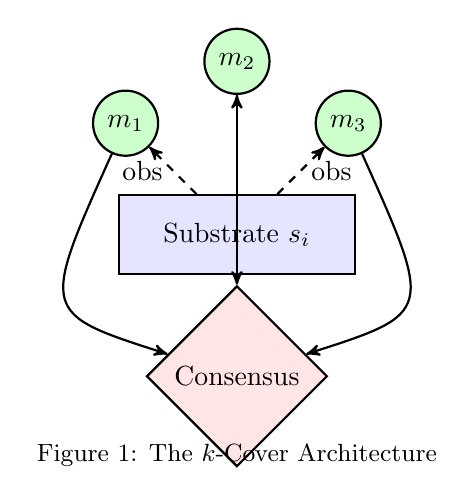
\begin{tikzpicture}[node distance=1.5cm, >=stealth', thick]
    % Substrate
    \node[draw, rectangle, fill=blue!10, minimum width=3cm, minimum height=1cm] (S) {Substrate $s_i$};
    
    % Monitors
    \node[draw, circle, fill=green!20, above left of=S, node distance=2cm] (M1) {$m_1$};
    \node[draw, circle, fill=green!20, above of=S, node distance=2.2cm] (M2) {$m_2$};
    \node[draw, circle, fill=green!20, above right of=S, node distance=2cm] (M3) {$m_3$};
    
    % Observation lines
    \draw[->, dashed] (S) -- (M1) node[midway, left] {obs};
    \draw[->, dashed] (S) -- (M2);
    \draw[->, dashed] (S) -- (M3) node[midway, right] {obs};
    
    % Consensus/Actuator
    \node[draw, diamond, fill=red!10, below of=S, node distance=1.8cm] (C) {Consensus};
    \draw[->] (M1) .. controls (-2.5,-1) .. (C);
    \draw[->] (M2) -- (C);
    \draw[->] (M3) .. controls (2.5,-1) .. (C);
    
    \node[below of=C, node distance=1cm] {\small Figure 1: The $k$-Cover Architecture};
\end{tikzpicture}
\end{figure}

The $k$-cover ensures that even if $k-1$ monitors are compromised or noisy, the system still receives a signal regarding its viability. This is the mathematical basis for the robustness seen in biological networks and legal checks-and-balances.

\section{Ratcheted Advancement}
A persistent system does not merely stay safe; it grows. However, growth is risky. To prevent collapse, growth must be ``ratcheted.''

\begin{theorem}[The Ratcheted Frontier]
A system may only increase its viability floor $\underline{s}_i \to \underline{s}_i + \Delta$ if the new state is certified to be within the \textbf{Viability Kernel} $\text{Viab}(K)$, ensuring that a control law exists to keep the system safe indefinitely from the new floor.
\end{theorem}



\begin{figure}[h]
\centering
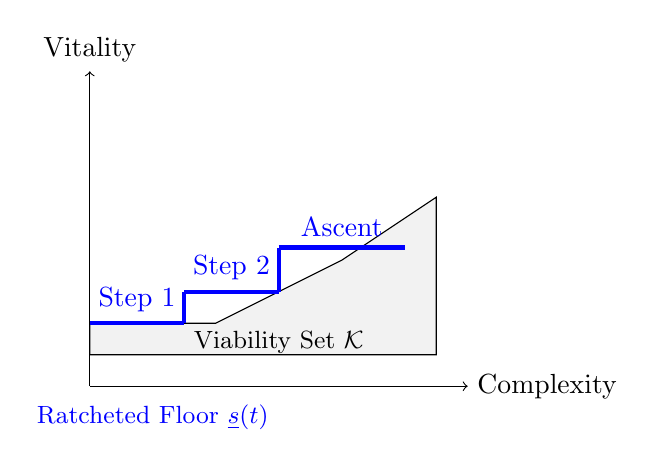
\begin{tikzpicture}[scale=0.8]
    % Axes
    \draw[->] (0,0) -- (6,0) node[right] {Complexity};
    \draw[->] (0,0) -- (0,5) node[above] {Vitality};
    
    % Safe set
    \draw[fill=gray!10] (0,1) -- (2,1) -- (4,2) -- (5.5,3) -- (5.5,0.5) -- (0,0.5) -- cycle;
    \node at (3,0.7) {\small Viability Set $\mathcal{K}$};
    
    % Ratchet Steps
    \draw[ultra thick, blue] (0,1) -- (1.5,1) node[midway, above] {Step 1};
    \draw[ultra thick, blue] (1.5,1) -- (1.5,1.5);
    \draw[ultra thick, blue] (1.5,1.5) -- (3,1.5) node[midway, above] {Step 2};
    \draw[ultra thick, blue] (3,1.5) -- (3,2.2);
    \draw[ultra thick, blue] (3,2.2) -- (5,2.2) node[midway, above] {Ascent};
    
    % Labels
    \node[blue] at (1,-0.5) {\small Ratcheted Floor $\underline{s}(t)$};
\end{tikzpicture}
\end{figure}

\section{The Chain Reaction of Persistence}
The most critical result of our framework is the \textbf{Stability-Momentum Coupling}. As substrates become more secure (efficiency), the resources available for monitoring increase (feedback). This improves the precision of the $k$-cover, which in turn allows for a higher rate of ratcheted advancement. 

This feedback loop creates a ``Chain Reaction'' where complexity bootstraps itself. Systems that enter this loop undergo an ``Inevitable Ascent.''



\section{From SCAP to Recursive Viability}
In previous iterations, we referred to the internal alignment of intelligence as the \textit{Sustainable Collaborative Alignment Principle}. We now formalize this as \textbf{Recursive Viability}. 

When an intelligent system models its own dependencies, its internal ``Learning Loop'' ($L$) becomes a substrate itself. To persist, the system must apply the same $k$-cover monitoring to its own objectives and learning processes as it does to its physical energy sources. Alignment is therefore not a constraint imposed on intelligence, but a structural requirement for its continued existence.

\section{Conclusion}
The ascent toward complexity is a mathematical necessity for duration. By viewing AI safety and institutional design through the lens of $k$-covers and ratcheted kernels, we move from speculative ethics to rigorous engineering. Persistence is the reward for systems that learn to monitor what they stand on.

\end{document}